
\begin{appendices}
	\section{\lr{Modified Anton's measure}}
	\label{ModifiedMeasure}
	\begin{itemize}
		\item 
		فرمول استفاده شده در مقاله
		\lr{\cite{AntonPolk}}
		\begin{equation}
			\text{Overlap}_{Sum}(i, j) = \frac{\sum_{f = 1}^{F} (S^f_{i,t}P_{i,t}+S^f_{j,t}P_{j,t})}{S_{i,t}P{i,t} + S_{j,t}P{j,t}}
			\label{Sum}
		\end{equation}
		\item 
		این فرمول توزیع مالکیت را در نظر نمیگیرد و فقط جمع ساده است
		\item
		وزن دهی دوباره انجام دادیم و دو فرمول زیر را پیشنهاد می دهیم	
		\item
		
		\begin{equation}
			\text{Overlap}_{Sqrt}(i, j) =  [\frac{\sum_{f =1}^{F}(\sqrt{S^f_{i,t}P_{i,t}}+\sqrt{S^f_{j,t}P_{j,t}})}{\sqrt{S_{i,t}P{i,t}} + \sqrt{S_{j,t}P{j,t}}}]^2 
			\label{sqrt}
		\end{equation}
		
		\begin{equation}
			\text{Overlap}_{Quadratic}(i, j) =  [{\frac{\sum_{f = 1}^{F}[(S^f_{i,t}P_{i,t})^2+(S^f_{j,t}P_{j,t})^2]}{(S_{i,t}P{i,t})^2 + (S_{j,t}P{j,t})^2}}]^{-1}
			\label{Quadratic}
		\end{equation}
		\item
		تفسیر این دو ملاک عبارت است از این که در صورت تقسیم دو شرکت به صورت مساوی بین n مالک، این ملاک عدد n را نشان می دهد
		\LR{\footnote{ \tiny
				Each holder owns $ 1/n $ of each firm ,Firm's market cap is $ \alpha_1 $ and $ \alpha_2 $, So for each holder of firms we have $ S^f_{i,t}P_{i,t} = \alpha_i/n $\\
				$
				[  \frac{\sum_{f=1}^{n} \sqrt{\alpha_1/n}+\sum_{f=1}^{n} \sqrt{\alpha_2/n}}{\sqrt{\alpha_1} + \sqrt{\alpha_2}}]^2 
				= [\frac{\sqrt{n}(\sqrt{\alpha_1} +\sqrt{\alpha_2 })}{\sqrt{\alpha_1} + \sqrt{\alpha_2}}]^2 = n $
				\\
				$
				[\frac{\sum_{f=1}^{n} {(\alpha_1/n)^2}+\sum_{f=1}^{n} {(\alpha_2/n)^2}}{\alpha_1^2 +{\alpha_2}^2}]^{-1} = [\frac{{\alpha_1^2 + \alpha_2^2 }}{n(\alpha_1^2 + \alpha_2^2)}]^{-1} = n
				$
		}}
		\item
		در واقع یعنی تعداد مالک مشترک مساوی دو شرکت را تولید می کند
	\end{itemize}
	
	\begin{itemize}
		\item 
		مثال عددی برای مقایسه دو ملاک معرفی شده
		\begin{itemize}
			\item 
			دو شرکت x و y با یک مالک مشترک با مالکیت 
			$ \alpha $ 
			و
			$ \beta $
			از مارکت کپ دو شرکت با ارزش یکسان.
			شکل 
			\ref{gExample1}
			\begin{itemize}
				\item 
				برای سادگی فرق می کنیم
				($ \alpha + \beta  = 100$)
				\item شکل مثال
				\begin{figure}[htbp]
					\centering
					\caption{\lr{ Numeric example 1} }
					\label{gExample1}
					\begin{tikzpicture}[node distance=1cm]
						
						\node (Firm) [startstop3] {\tiny Firm X};
						\node (Firm2) [startstop3,right of = Firm  , xshift=-5.5cm ] {\tiny Firm Y};
						\node (Owner) [startstop3,right of = Firm , yshift=1cm , xshift=-3.25cm ] {\tiny Common owner };
						
						
						\draw[arrow] (Owner) -- node[sloped, anchor=center, above] {\tiny $ \alpha $} (Firm) ;
						
						\draw[arrow] (Owner) -- node[sloped, anchor=center, above] {\tiny $ \beta $} (Firm2) ;
						%
						%\node() at (3,0)
						%    {$ \alpha + \beta = 100 $}; 
					\end{tikzpicture}
				\end{figure}\bigskip
				\item
				شکل 
				\ref{example1Results}
				نتایج محاسبات را نشان می دهد
				\item
				\begin{figure}[htbp]
					\caption{ \lr{Comparison of three measure for common ownership}}
					\label{example1Results}
					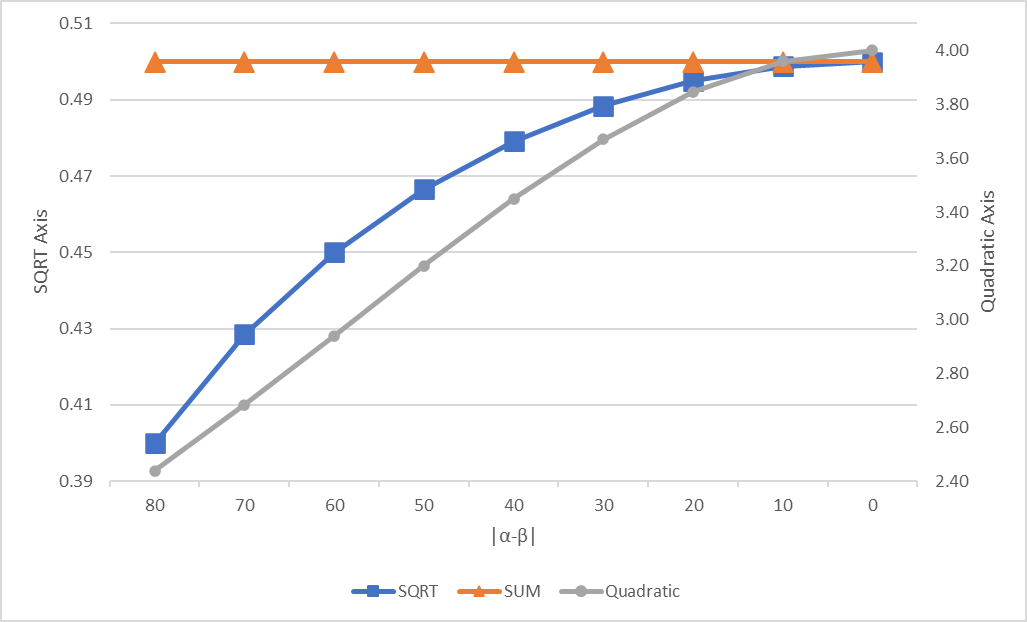
\includegraphics[width=0.47\linewidth]{1.png}
					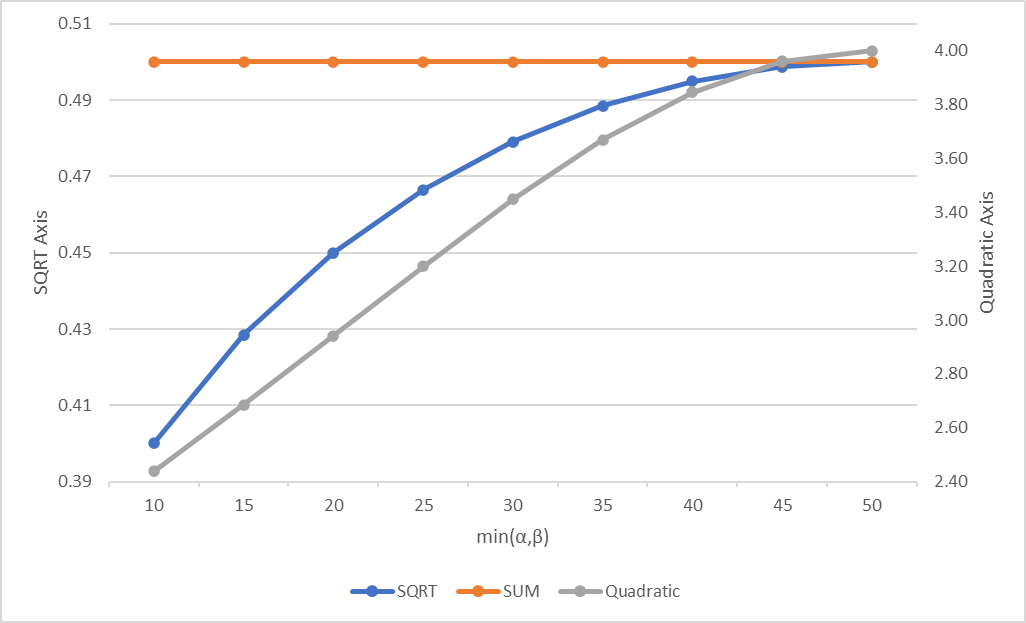
\includegraphics[width=0.47\linewidth]{2.png}
				\end{figure}
				\item
				ملاک اصلی برای هر توزیعی ثابت است ولی دو ملاک معرفی شده تفاوت را ایجاد کرده است
				\item
				مالکیت مشترک در حال 50-50 بیشترین و در حال 10-90 کمترین حالت ممکن است 
				
				
			\end{itemize}
			\item 
			حال در مثال قبل فرض کنید سه مالک مشترک داریم که در برای مالک 1 مالکیت در شرکت x و y عبارت است از 
			$\alpha_1$ 
			و
			$\beta_1$
			
			\begin{itemize}
				\item 
				شکل مثال
				\begin{figure}[htbp]  \centering
					\caption{ Numeric example 2}
					\label{gExample2}
					\centering
					\begin{tikzpicture}[node distance=1cm]
						
						
						\node (Firm) [startstop3] {\tiny Firm X};
						\node (Firm2) [startstop3,right of = Firm , yshift=0cm , xshift=-8cm ] {\tiny Firm Y};
						
						\node (Owner) [startstop3,above of = Firm , yshift=1.25cm , xshift=-3.5cm ] {\tiny Common owner 1 };
						
						
						\node (Owner2) [startstop3,right of = Firm , yshift= 0 , xshift=-4.5cm ] {\tiny Common owner 2 };
						
						\node (Owner3) [startstop3,below of = Firm , yshift=-1.25cm , xshift=-3.5cm ] {\tiny Common owner 3 };
						
						
						
						
						
						\draw [-latex] (Owner) to [bend right =0]  node[sloped, anchor=center, above] {\tiny $ \beta_1 $} (Firm2);
						
						\draw [-latex] (Owner) to [bend left =0]  node[sloped, anchor=center, above] {\tiny $ \alpha_1 $} (Firm);
						
						
						
						\draw [-latex] (Owner2) to [bend right =0]  node[sloped, anchor=center, below] {\tiny $ \beta_2 $} (Firm2);
						
						\draw [-latex] (Owner2) to [bend left =0]  node[sloped, anchor=center, below] {\tiny $ \alpha_2 $} (Firm);
						
						
						
						\draw [-latex] (Owner3) to [bend left =0]  node[sloped, anchor=center, below] {\tiny$ \beta_3 $} (Firm2);
						
						\draw [-latex] (Owner3) to [bend right =0]  node[sloped, anchor=center, below] {\tiny $ \alpha_3 $} (Firm);
						
						
						
					\end{tikzpicture}
				\end{figure}
				\item 
				نتایح در 
				\ref{Example2}
				نشان داده شده است
				\begin{LTR}
					\lr{\begin{table}[htbp]
							\centering
							\caption{ text}
							\label{Example2}
							\resizebox{1\textwidth}{!}
							{
								    \begin{tabular}{cccccccc}
    \hline\hline
        Ownership  & Type I & Type II & Type III & Type IV & Type V & Type VI & Type VII \\
          \hline
    $ \alpha_1 $    & 1/3 &20      &  10   & 20    & 10    & 5     & 1  \\
    $ \beta_1 $    & 1/3  & 10    & 10   & 20    & 10    & 5     & 1  \\
    $ \alpha_2 $    & 1/3  & 10    & 80    & 20    & 10    & 5     & 1 \\
    $ \beta_2 $    & 1/3  & 20    & 80    & 20    & 10    & 5     & 1  \\
    $ \alpha_3 $    & 1/3  & 70    & 10    & 20    & 10    & 5     & 1 \\
    $ \beta_3 $    & 1/3  & 70    & 10   & 20    & 10    & 5     & 1  \\
    \hline
    SQRT  & 3     &  2.56  & 2.33 & 1.8   & 0.9   & 0.45  & 0.09 \\
    SUM   & 1     & 1     & 1     & 0.6   & 0.3   & 0.15  & 0.03 \\
    Quadratic & 3     & 1.85  & 1.52  & 8.33  & 33.33 & 133.33 & 3333.33 \\
 
    \hline\hline
    \end{tabular}%
							}
					\end{table}}
				\end{LTR}
				\item 
				برای مالکیت های برابر تمام مارکت کپ تو شرکت نتایج با قبل یکسان است
				\item 
				ستون اول هم تفسیر ملاک را نشان می دهد که در صورت تقسیم شرکت به 3 مالک، عدد برابر 3 است
				\item 
				برای مالکیت های کمتر از 100 درصد ملاک درجه 2 مقادیر غیر واقعی تولید می کند
				\item 
				برای همین از ملاک جذری استفاده می کنیم
				
				
			\end{itemize}
			\item 
			حال فرض اصلی که ارزش بازاری دو شرکت برابر است را کنار می گذاریم برای مثال دو شرکت را با دو مالک مشترک در حالت های مختلف بررسی می کنیم
			
			
			\begin{itemize}
				\item 
				شکل 
				\ref{sqrtMarket}
				و
				\ref{sumMarket}
				نتایج را برای جمع ثابت مالکیت برای سه حالت توزیع مختلف رسم شده است
				
				\item 
				\begin{LTR}
					\lr{	\begin{figure}[htbp]
							\centering
							\caption{ SQRT measure for fixed aggregate ownership on different relative market cap ratios}
							\label{sqrtMarket}
							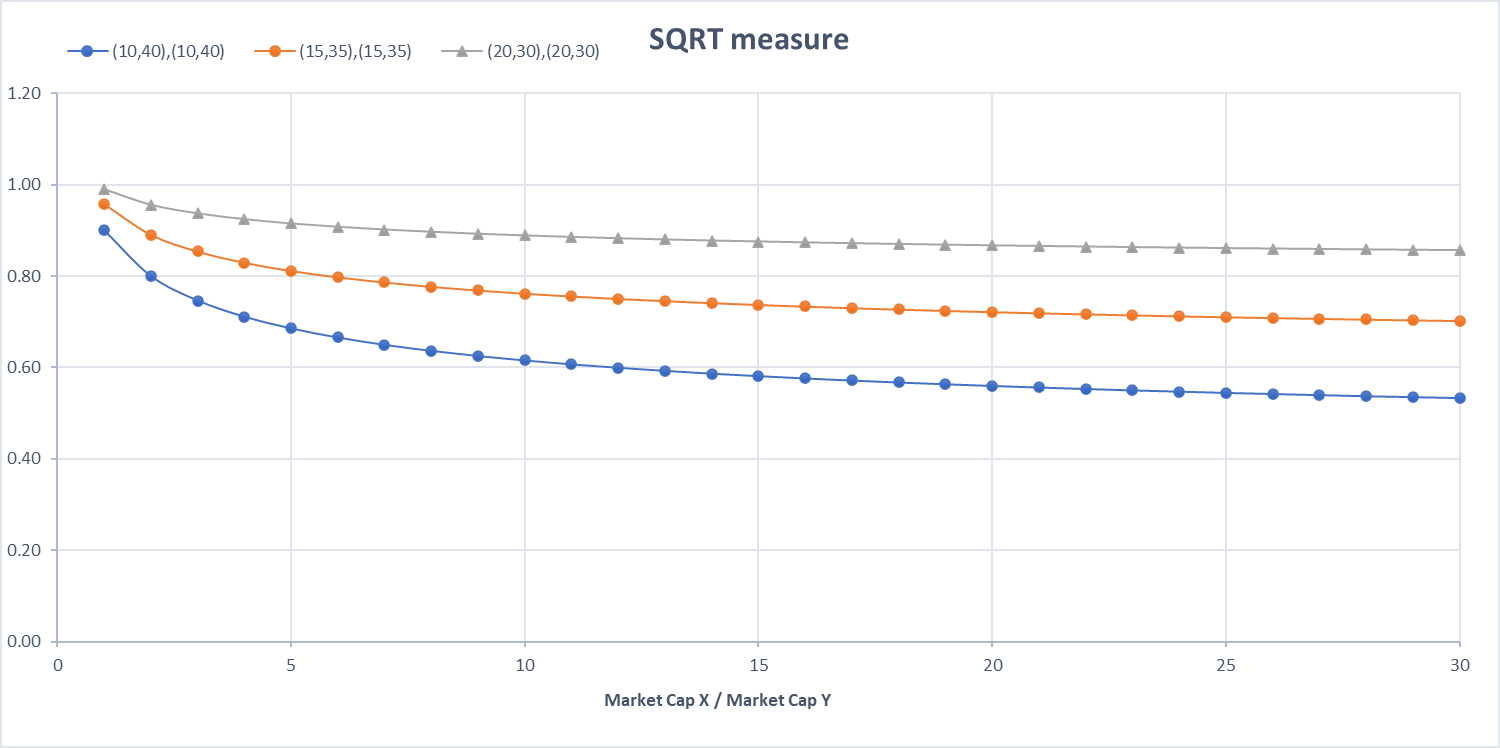
\includegraphics[width=0.85\linewidth]{3.png}
						\end{figure}
						\begin{figure}[htbp]
							\centering
							\caption{ Sum measure for fixed aggregate ownership on different relative market cap ratios}
							\label{sumMarket}
							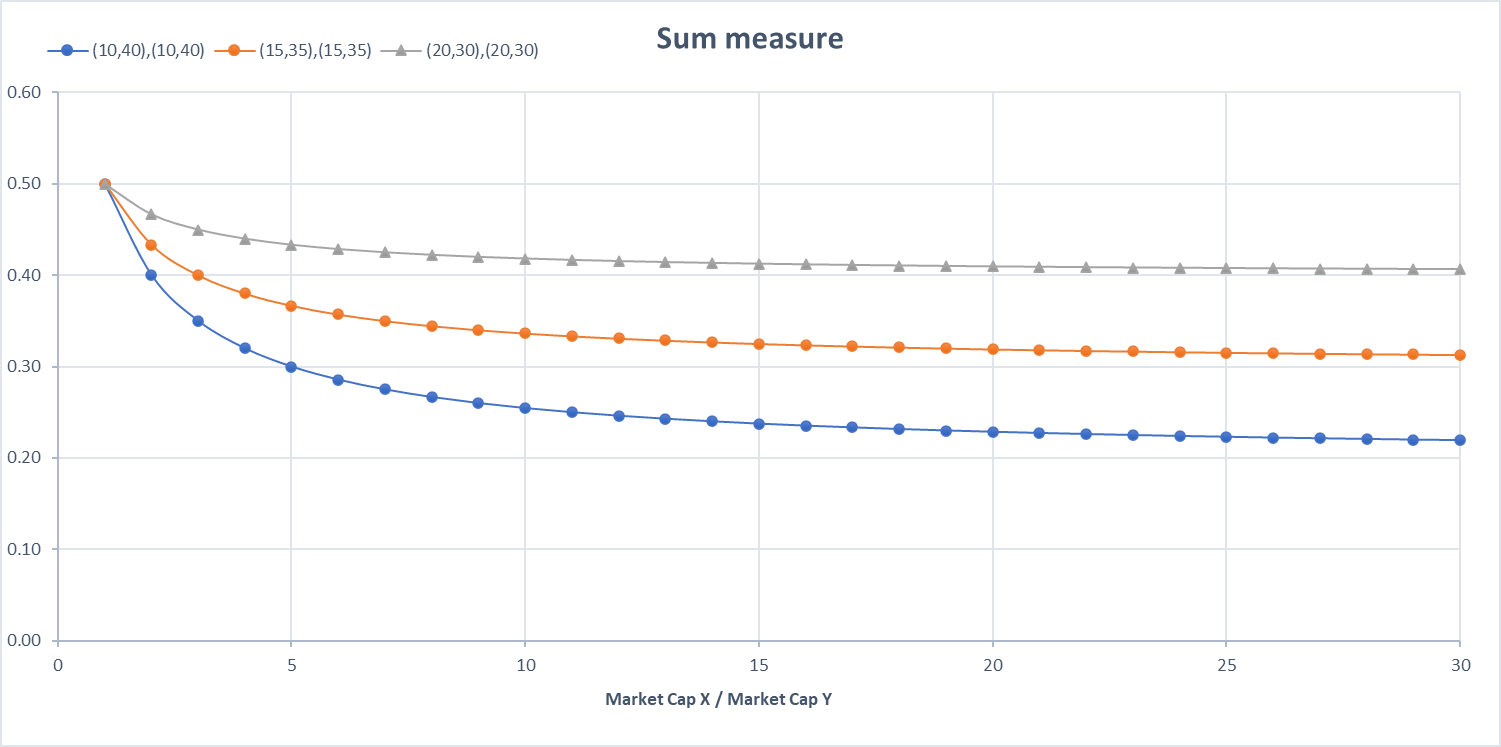
\includegraphics[width=0.85\linewidth]{4.png}
					\end{figure}}
				\end{LTR}
				\item 
				جدول 
				\ref{marketcap}
				نتایج محاسبات را نشان داده است.
				
				\item 
				\begin{LTR}
					\lr{\begin{table}[htbp]
							\centering
							\caption{text }
							\label{marketcap}
							\resizebox{!}{!}
							{
								          \scriptsize
    \begin{tabular}{ccccccc}
    \hline\hline
  & \multicolumn{6}{c}{\tiny($ \alpha_1 $,$ \beta_1 $),($ \alpha_2 $,$ \beta_2 $) }\\ \cmidrule(lr){2-7}
               & \multicolumn{2}{c}{\tiny(10,40),(10,40)} & \multicolumn{2}{c}{\tiny(15,35),(15,35)} & \multicolumn{2}{c}{\tiny(20,30),(20,30)} \\ \cmidrule(lr){2-3}\cmidrule(lr){4-5}\cmidrule(lr){6-7}
    \tiny $ \frac{\text{MarketCap}_x}{\text{MarketCap}_y} $     &\tiny SQRT  & \tiny SUM   &\tiny SQRT  &\tiny SUM   &\tiny SQRT  &\tiny SUM \\ 
     \hline\addlinespace

         1     & 0.90  & 0.50  & 0.96  & 0.50  & 0.99  & 0.50 \\
         2     & 0.80  & 0.40  & 0.89  & 0.43  & 0.96  & 0.47 \\
         3     & 0.75  & 0.35  & 0.85  & 0.40  & 0.94  & 0.45 \\
         4     & 0.71  & 0.32  & 0.83  & 0.38  & 0.92  & 0.44 \\
         5     & 0.69  & 0.30  & 0.81  & 0.37  & 0.91  & 0.43 \\
         6     & 0.67  & 0.29  & 0.80  & 0.36  & 0.91  & 0.43 \\
         7     & 0.65  & 0.28  & 0.79  & 0.35  & 0.90  & 0.43 \\
         8     & 0.64  & 0.27  & 0.78  & 0.34  & 0.90  & 0.42 \\
         9     & 0.63  & 0.26  & 0.77  & 0.34  & 0.89  & 0.42 \\
         10    & 0.62  & 0.25  & 0.76  & 0.34  & 0.89  & 0.42 \\
     
    \hline\hline
    \end{tabular}
							}
					\end{table}}
				\end{LTR}
				\item
				ملاک وزن دهی جذری به دلیل تغییرات بهتر و مقادیر معقول برای مقادیر کم مالکیت مشترک انتخاب شده است
			\end{itemize}
			
			
			
		\end{itemize}
	\end{itemize}
	
	
	
	
	
	
	
	
	
	
	
	
	
	\subsection{\lr{Common Ownership measure}}
	\begin{itemize}
		\item 
		برآورد مدل اصلی برای دو نوع اندازه گیری مالکیت مشترک
		\item 
		به شیوه قبلی
		\item 
		در نظر گرفتن توزیع سبب کاهش معناداری می شود که نشان می دهد بین حالت های مختلف توزیع تفاوت وجود دارد
		\item
		اثر در اندازه گیری جمع ساده بیش از اندازه برآور می شد
		
	\end{itemize}
	
	{\begin{table}[htbp]
			%	\centering
			\caption{Connected Co-movement}
			\label{mresult2Polk}
			\resizebox{1\textwidth}{!}{
				\begin{LTR}
					\lr{{
\def\sym#1{\ifmmode^{#1}\else\(^{#1}\)\fi}
\begin{tabular}{l*{8}{c}}
\hline\hline
                &\multicolumn{8}{c}{Dependent Variable: Future Monthly Correlation of 4F+Industry Residuals}                                                            \\\cmidrule(lr){2-9}
                &\multicolumn{1}{c}{(1)}         &\multicolumn{1}{c}{(2)}         &\multicolumn{1}{c}{(3)}         &\multicolumn{1}{c}{(4)}         &\multicolumn{1}{c}{(5)}         &\multicolumn{1}{c}{(6)}         &\multicolumn{1}{c}{(7)}         &\multicolumn{1}{c}{(8)}         \\
\hline
Common Ownership Measure&  0.00370\sym{***}&  0.00325\sym{***}&  0.00155\sym{*}  &  0.00109         & 0.000333         &-0.000105         & 0.000550         & 0.000283         \\
                &   (5.58)         &   (4.97)         &   (2.61)         &   (1.84)         &   (0.54)         &  (-0.17)         &   (1.07)         &   (0.58)         \\
[1em]
SameGroup       &                  &                  &   0.0229\sym{***}&   0.0234\sym{***}&   0.0100\sym{**} &   0.0103\sym{**} &  0.00626         &  0.00668         \\
                &                  &                  &   (7.89)         &   (7.93)         &   (3.26)         &   (3.17)         &   (1.79)         &   (1.79)         \\
[1em]
 $ \text{\small Common Ownership Measure} \times {\text{SameGroup} }$ &                  &                  &                  &                  &   0.0134\sym{***}&   0.0135\sym{***}&   0.0127\sym{***}&   0.0126\sym{***}\\
                &                  &                  &                  &                  &   (9.47)         &  (10.65)         &   (9.23)         &   (9.71)         \\
\hline
Observations    &   398818         &   398818         &   398818         &   398818         &   398818         &   398818         &   398818         &   398818         \\
Group FE        &       No         &       No         &       No         &       No         &       No         &       No         &      Yes         &      Yes         \\
Measurement     &      Sum         &      Sum         &      Sum         &      Sum         &      Sum         &     SQRT         &      Sum         &     SQRT         \\
$ R^2 $         &  0.00433         &  0.00427         &  0.00518         &  0.00515         &  0.00554         &  0.00551         &   0.0182         &   0.0182         \\
\hline\hline
\multicolumn{9}{l}{\footnotesize \textit{t} statistics in parentheses}\\
\multicolumn{9}{l}{\footnotesize \sym{*} \(p<0.05\), \sym{**} \(p<0.01\), \sym{***} \(p<0.001\)}\\
\end{tabular}
}
}
				\end{LTR}
			}
	\end{table}}
	
	\FloatBarrier
	
	
	
	
	
	\FloatBarrier
	
	
	
	\section{\lr{Overview of Business Groups in Tehran Stock Exchange}} \label{BGDef}
	
	\begin{itemize}
		\item 
		گروه های کسب و کار در کشور های در حال توسعه و توسعه یافته وجود دارد
		
		\lr{\cite{Khanna2007}}
		\item 
		گروه کسب و کار مجموعه ای از شرکت های به هم پیوسته است که از لحاظ قانونی غیروابسطه هستند ولی ارتباطات رسمی از طریق برای مثال سرمایه و غیر رسمی مانند فامیلی دارند
		\item 
		در چین و ایران گروه های کسب و کار مرتبط با حاکمیت هستند
		
		\item 
		لایه های پیچیده و تو در توی مالکیت در ایران وجود دارد 
		
		\lr{\cite{FirmInterlock}}
		\item 
		دلیل اصلی بسیاری از گروه های کسب و کار در ایران انفلاب سال 
		1375 می باشد
		
		\lr{\cite{Aliabadi2022}}
		\begin{itemize}
			\item 
			بسیاری از شرکت های قبل از انقلاب دولتی شدند
			\item 
			بخشی از شرکت های حاضر در صنایع نیز توسط IDRO ایجاد شده است
			\item 
			در ادامه فاز های متوالی خصوصی سازی توسط دولت در بازار سرمایه  بوده است
			\begin{itemize}
				\item 
				در فاز اول خصوصی سازی حدود 300 شرکت خصوصی شده اند
				\item 
				در فاز دوم حدودا 150 مییارد دلار از شرکت های دولتی خصوصی شدند 
				\item 
				صندوق های بازنشستگی، موسسات نظامی، موسسات فرهنگی و دینی و موسسات انقلابی مشتری های اصلی مرحله دوم خصوصی سازی بوده اند
				\item 
				در این فاز بسیاری از  گروه های کسب و کار تشکیل شده اند و شرکت ها از دولتی به شبه دولتی تبلدیل شده اند	
			\end{itemize}
		\end{itemize}	
		\item
		فاز های خصوصی سازی و گسترش بازار سرمایه ایران سبب تغییر ساختار مالکیت در شرکت های قبل از انقلاب و موسسات بعد از انفلاب شده است
		\item
		سبب ایجاد گروه های کسب و کار بزرگ شده است که بسیاری از صنایع و شرکت ها را مدیریت می کنند
		
	\end{itemize}
	
	\begin{itemize}
		\item 
		انتظار داریم شرکت ها حاضر در گروه های کسب و کار در یک صنعت حضور داشته باشند
		\begin{itemize}
			\item 
			38\% جفت های شناسایی شده در یک گروه کسب و کار در یک صنعت قرار دارند 
			\item 
			تنها 5\% جفت های شناسایی شده بیرون یک گروه کسب و کار در یک صنعت قرار دارند 
			\begin{figure}[htbp]
				\caption{}
				\label{sameIndustryinBG}
				\centering
				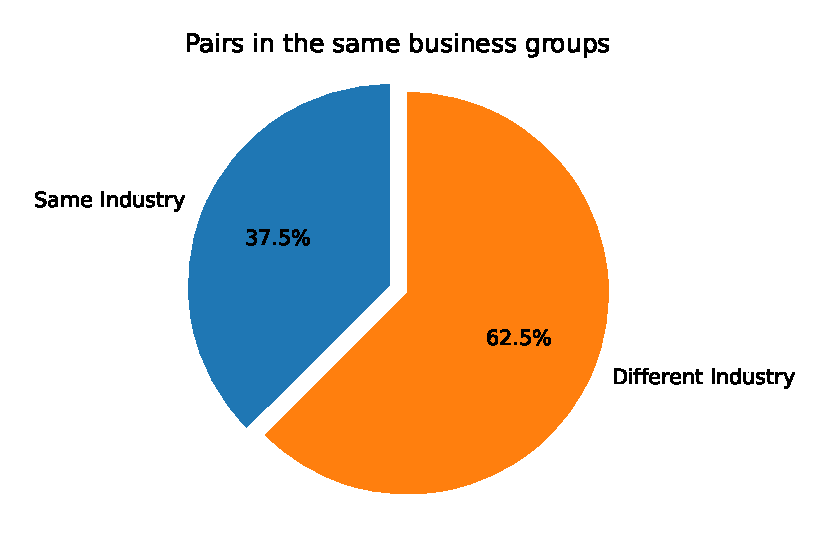
\includegraphics[width=0.48\linewidth]{Output/sameIndustryinBG.eps}
				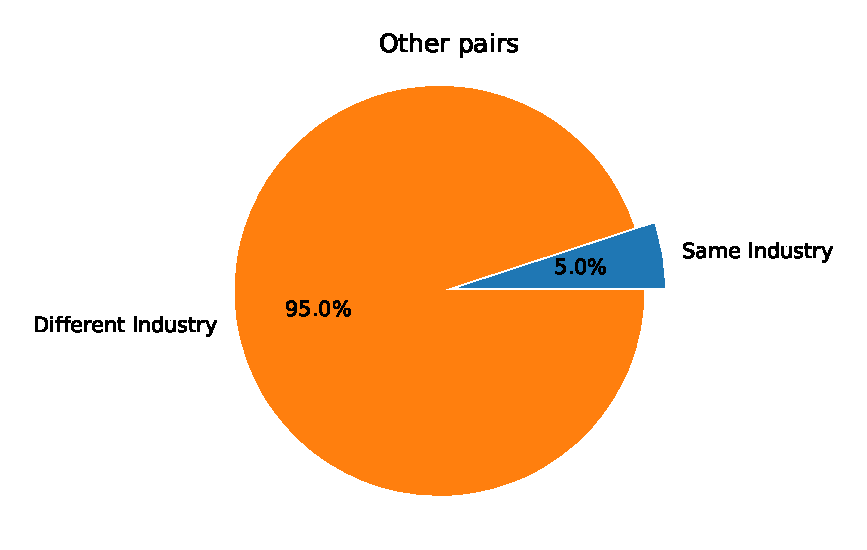
\includegraphics[width=0.48\linewidth]{Output/sameIndustryNoinBG.eps}
			\end{figure}
			\item 
			از نظر اندازه و نسبت بوک تو مارکت ججفت های گروه های کسب و کار شبیه جامعه هستند
			\item 
			همانطور که قبلا هم گفتیم متوسط مالکیت مشترک در گروه های کسب و کار زیاد است
			\item 
			شکل 
			\ref{BGSummary}
			خلاصه ها را نشان داده است
			\begin{figure}[htbp]
				\caption{}
				\label{BGSummary}
				\centering
				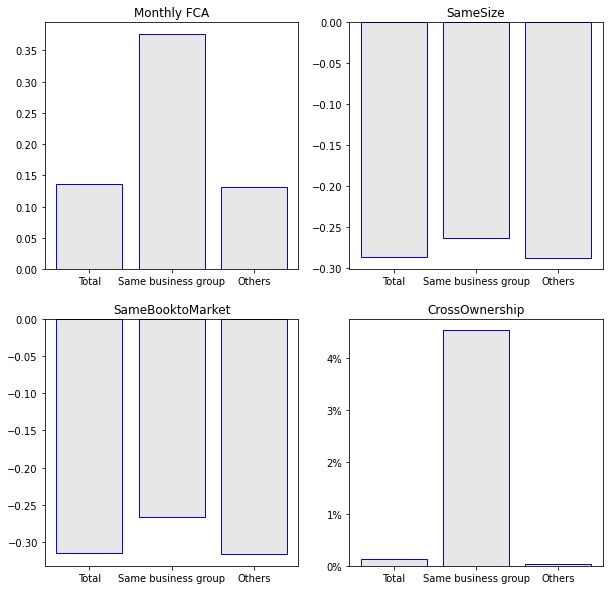
\includegraphics[width=0.85\linewidth]{Output/BGSummary.eps}
			\end{figure}
		\end{itemize}
		
		
	\end{itemize}
	
	
	\FloatBarrier
	
	
	
	
	
\end{appendices}
